\documentclass[areasetadvanced]{scrartcl}

\usepackage[utf8]{inputenc}
\usepackage[T2A]{fontenc}
\usepackage[english,russian]{babel}
\usepackage[footskip=1cm,left=25mm, right=15mm, top=20mm, bottom=20mm]{geometry}
\usepackage{setspace}
\usepackage{amsmath, amssymb}  
\usepackage{graphicx}
\usepackage[final]{pdfpages}
\usepackage{ragged2e}
\usepackage{tikz}
\usetikzlibrary{arrows.meta}
\usepackage{float}
\usepackage{dashrule}
\usepackage{lipsum}
\pagestyle{plain} 
\usepackage{fancyhdr} 
\usepackage{hyperref} 
\usepackage{parskip}
\usepackage{textcomp, enumitem}
\usepackage{indentfirst}
\usepackage{graphicx}
\usepackage{pdflscape}
\usepackage{algorithm}
\usepackage{algpseudocode}
\usepackage{array}  
\usepackage{geometry}
\usepackage{afterpage}
\usepackage{minted}
\setcounter{secnumdepth}{3}  
\setcounter{tocdepth}{3}     
\usepackage{listings} 
\setlength{\parindent}{1.25cm}
\tikzstyle{block} = [rectangle, rounded corners, minimum width=3cm, minimum height=1cm, text centered, draw=black, fill=lightgray]

\setkomafont{sectioning}{\normalfont\bfseries} % для заголовков разделов и подразделов
\setkomafont{section}{\normalfont\Large\bfseries}
\setkomafont{subsection}{\normalfont\large\bfseries}
\setkomafont{subsubsection}{\normalfont\large\bfseries}
\setkomafont{paragraph}{\normalfont\large\bfseries} % для заголовков параграфов (если они есть)

\lstset{
  language=C++,
  basicstyle=\ttfamily\small,
  keywordstyle=\color{blue}\bfseries,
  stringstyle=\color{red},
  commentstyle=\color{green!70!black},
  numbers=left,
  numberstyle=\tiny,
  stepnumber=1,
  numbersep=10pt,
  showstringspaces=false,
  breaklines=true,
  frame=single
}

\setcounter{tocdepth}{3}
\begin{document}
\sloppy
	\thispagestyle{empty}
	\begin{center}
		\large{МИНОБРНАУКИ РОССИИ} \par
		\vspace{0.3cm}
		\normalsize
		{ФЕДЕРАЛЬНОЕ ГОСУДАРСТВЕННОЕ АВТОНОМНОЕ ОБРАЗОВАТЕЛЬНОЕ УЧРЕЖДЕНИЕ ВЫСШЕГО ОБРАЗОВАНИЯ} \par
		\vspace{0.3cm}
		\textbf{\guillemotleft САНКТ-ПЕТЕРБУРГСКИЙ ПОЛИТЕХНИЧЕСКИЙ}
		\textbf{УНИВЕРСИТЕТ ПЕТРА ВЕЛИКОГО\guillemotright} \par
		\vspace{0.3cm}
		{Институт компьютерных наук и кибербезопасности}\par
		{Высшая школа технологий искусственного интеллекта}\par
	\end{center}
	\vfill
	\begin{center}
		{\large Отчёт по дисциплине \guillemotleft Математическая логика\guillemotright}\par
		{\huge   Лабораторная работа №4
		
		\guillemotleft Доработка компилятора CMiLan\guillemotright}\par
            {\huge Вариант \textbf{Цикл for. Тип №2.}}
         
	\end{center}
	\vfill
	\begin{flushleft}
		Студент: \hspace{1.8cm} \rule[0pt]{2.5cm}{0.5pt}\hfill Салимли Айзек Мухтар Оглы\par
		\vspace{1.5cm}
		Преподаватель: \hspace{0.55cm} \rule[0pt]{2.5cm}{0.5pt}\hfill  Востров Алексей Владимирович
	\end{flushleft}
	\vspace{0.5cm}
	\begin{flushright}
		\guillemotleft \rule[0pt]{0.8cm}{0.5pt}\guillemotright \rule[0pt]{2cm}{0.5pt} 20\rule[0pt]{0.5cm}{0.5pt} г.
	\end{flushright}
	\vfill
	\begin{center}
		Санкт-Петербург, 2025
	\end{center}
	\newpage
	\tableofcontents
	\newpage

    \section*{Введение}
    \addcontentsline{toc}{section}{Введение}
    Язык \emph{Милан} --- учебный процедурный язык программирования.  
    В исходной версии компилятор \textbf{CMilan} поддерживал циклическую конструкцию
    \texttt{while}, но отсутствовал удобный счётный цикл.  
    В данной лабораторной работе компилятор расширен за счёт
    реализации оператора цикла
    
    \begin{center}
    \verb|for <идент> := <нач>, <кон> [, <итерация>] do <список_операторов> od|
    \end{center}
    
    Шаг не обязателен; если он опущен, используется значение \texttt{1}.  
    Задача потребовала изменить исходный C++-код компилятора \textbf{CMilan}.
    Были решены следующие подзадачи:
    \begin{itemize}
      \item расширить лексический анализатор (добавить ключевое слово
            \verb|for| и символ `\verb|,|`);
      \item дополнить грамматику языка;
      \item реализовать разбор цикла в синтаксическом анализаторе
            с одновременной генерацией p-кода;
      \item протестировать компилятор и виртуальную машину.
    \end{itemize}

    \newpage
    \section{Математическое описание}
    \subsection{Лексический и синтаксический анализ}
    Лексический анализатор – первый из "слоев" компилятора, отвечающий за выделение лексем для последующей обработки. Лексема – минимальная единица некоего словаря, представляющего наш язык. В роли лексемы могут служить служебные слова, операторы, идентификаторы и так далее. На Рис.1 представлена схема лексического анализатора. 

    \begin{figure}[H]
        \centering
        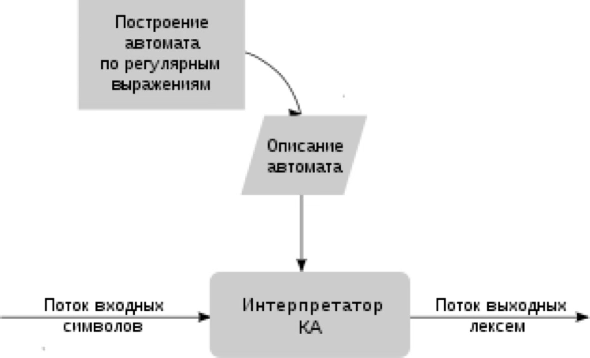
\includegraphics[width=0.5\textwidth]{schema.png}
        \caption{Схема лексического анализатора}
    \end{figure}

    Синтаксический анализ — процесс сопоставления линейной последовательности лексем естественного или формального языка с его формальной грамматикой. Результатом обычно является дерево разбора. Обычно применяется совместно с лексическим анализом.
    Синтаксический анализатор выражений (парсер) — часть программы, выполняющая чтение и анализ выражения. 
    Существует два типа алгоритмов синтаксического анализа: нисходящий и восходящий:
    \begin{itemize}
        \item Нисходящий парсер — продукции грамматики раскрываются, начиная со стартового символа, до получения требуемой последовательности токенов. 
        \item Восходящий парсер — продукции восстанавливаются из правых частей, начиная с токенов и кончая стартовым символом. 
    \end{itemize}

    Грамматика языка Милан использует нисходящий парсер. При восстановлении синтаксического дерева при нисходящем разборе слева направо последовательно анализирует все поддеревья, принадлежащие самому левому нетерминалу. Когда самым левым становится другой нетерминал, анализируется уже он.
    Компилятор языка Милан представляет собой транслятор, использующий метод рекурсивного спуска, и генератор p-кода. На Рис. 2 представлена полная схема компилятора Милан. 

    \begin{figure}[H]
        \centering
        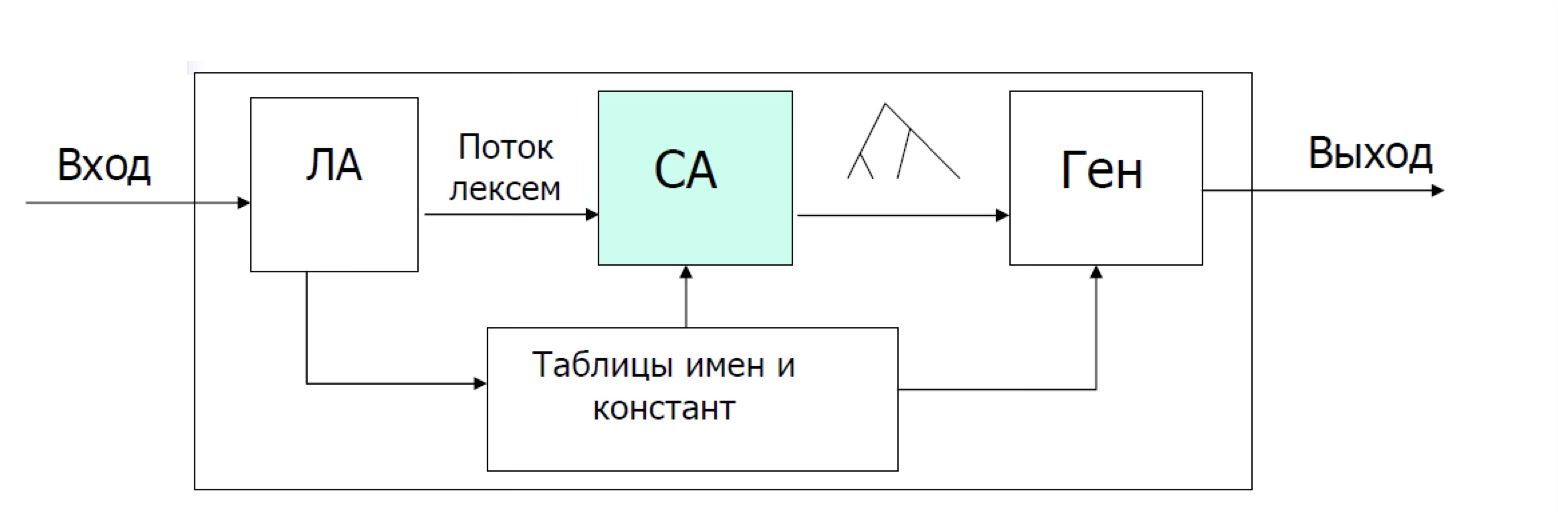
\includegraphics[width=0.8\textwidth]{compiler.png}
        \caption{Схема компилятора Милан}
    \end{figure}

    Грамматика языка Милан является LL(1) грамматикой, так как необходимо просмотреть поток всего на один символ вперед при принятии решения о том, какое правило грамматики необходимо применить. Грамматика языка Милан является контекстно-свободной, так как удовлетворяет определению КС-грамматики, т.е. продукции грамматики имеют вид $A \rightarrow \alpha$, где $A$ — одиночный нетерминал, а $\alpha$ — произвольная цепочка из терминалов и нетерминалов. Ниже представлена грамматика языка Милан. 

\[
\begin{aligned}
&\text{Prog} \rightarrow \textbf{begin}\ L\ \textbf{end} \\
&L \rightarrow S\ \mid\ L\ ;\ S \\
&S \rightarrow i_k := E \\
&\quad\;\;\;\mid\ \textbf{while}\ B\ \textbf{do}\ L\ \textbf{od} \\
&\quad\;\;\;\mid\ \textbf{if}\ B\ \textbf{then}\ L\ \textbf{fi} \\
&\quad\;\;\;\mid\ \textbf{if}\ B\ \textbf{then}\ L\ \textbf{else}\ L\ \textbf{fi} \\
&\quad\;\;\;\mid\ \textbf{write}\ (E) \\
&B \rightarrow E\ q_k\ E \\
&E \rightarrow E\ aop_k\ T\ \mid\ T \\
&T \rightarrow T\ mop_k\ P\ \mid\ P \\
&P \rightarrow i_k\ \mid\ c_k\ \mid\ (E)\ \mid\ \textbf{read} \\
\end{aligned}
\]

    \section{Синтаксические диаграммы}
    Ниже представлены синтаксические диаграммы для модифицированной грамматики языка Милан. Синтаксические диаграммы соответствуют расширенной БНФ-нотации грамматики языка Милан, каждому нетерминалу соответствует своя синтаксическая диаграмма. 

    \begin{figure}[H]
        \centering
        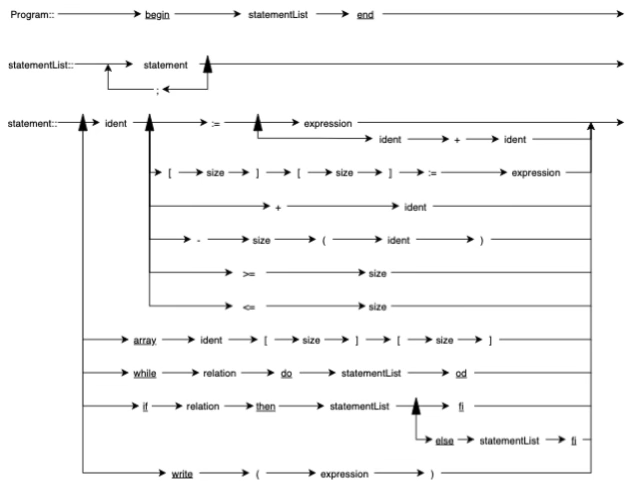
\includegraphics[width=0.8\textwidth]{beginEnd.png}
        \caption{Синтаксическая диаграмма}
    \end{figure}

    \begin{figure}[H]
        \centering
        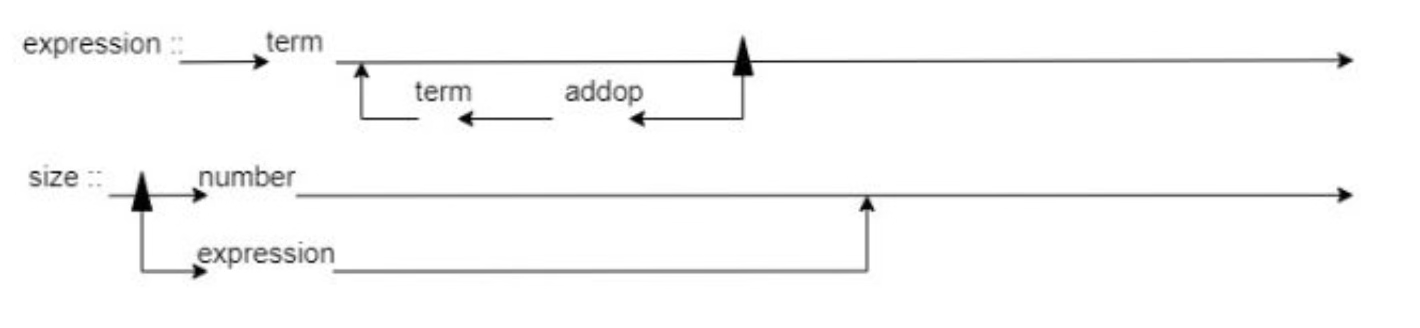
\includegraphics[width=0.8\textwidth]{Term.png}
        \caption{Синтаксическая диаграмма для Term}
    \end{figure}

    Первая синтаксическая диаграмма соответствует продукции начального нетерминала (ключевые слова 'begin' и 'end' отвечают за начало и конец программы соотвественно). Между границами программы находится тело программы (продукция statementList, вторая диаграмма), которая может включать в себя одну или более строк, разделенных знаком ';'.
    
Синтаксическая диаграмма для реализованного цикла for представлена ниже.

\begin{figure}[H]
    \centering
    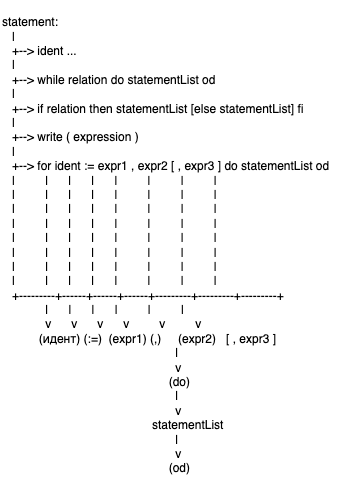
\includegraphics[width=0.5\textwidth]{diagram2.png}
    \caption{Синтаксическая диаграмма после добавления for}
\end{figure}

    \newpage
    \section{Компилятор \textbf{CMilan}}
    Компилятор состоит из трёх основных компонент:
    \begin{enumerate}
      \item \emph{лексический анализатор} (файл \lstinline{scanner.*});
      \item \emph{синтаксический анализатор} — рекурсивный нисходящий
            LL(1)-парсер (\lstinline{parser.*});
      \item \emph{генератор кода} для стековой виртуальной машины
            (\lstinline{codegen.*}).
    \end{enumerate}
    
    Лексер разбивает исходный текст на лексемы (\texttt{Token}),
    удаляя пробелы и комментарии.
    Парсер, получая поток лексем, проверяет его соответствие грамматике
    и одновременно формирует последовательность команд
    виртуальной машины (p-код).
    Так как грамматика Милана — LL(1), достаточно просмотра
    одного символа вперёд.
    
   % -----------------------------------------------------------------
   \newpage
\section{Формальная грамматика языка после расширения}
\subsection{Определение КС-грамматики}

Расширенный язык задаётся КС-грамматикой
$G=\langle N,\Sigma,P,S\rangle$.

\begin{itemize}
  \item $N=\{\langle program\rangle,\langle statementList\rangle,
            \langle statement\rangle,\langle expression\rangle,
            \langle term\rangle,\langle factor\rangle,
            \langle relation\rangle\}$.
  \item $\Sigma$ содержит все терминалы: ключевые слова \\
        $\{\texttt{begin,end,if,then,else,fi,while,do,od,for,write,read}\}$, \\
        служебные символы \texttt{‘:=’ ‘,’ ‘(’ ‘)’ ‘;’}  
        и множество идентификаторов/чисел.
  \item $S=\langle program\rangle$.
  \item $P$ приведено в БНФ ниже (дополнения выделены \textbf{жирным}).
\end{itemize}

\subsection{БНФ (расширенная)}

\begin{verbatim}
<program>       ::= 'begin' <statementList> 'end'

<statementList> ::= <statement> ';' <statementList>
                  | <statement>

<statement>     ::= <ident> ':=' <expression>
                  | 'if' <relation> 'then' <statementList>
                        ['else' <statementList>] 'fi'
                  | 'while' <relation> 'do' <statementList> 'od'
                  | **'for' <ident> ':=' <expression> ',' <expression>
                        [',' <expression>] 'do' <statementList> 'od'**
                  | 'write' '(' <expression> ')'

<expression>    ::= <term> { <addop> <term> }
<term>          ::= <factor> { <mulop> <factor> }
<factor>        ::= <number>
                  | <ident>
                  | '(' <expression> ')'
                  | '-' <factor>
                  | 'read'

<relation>      ::= <expression> <cmp> <expression>
\end{verbatim}
\newpage
\section{Грамматика LL(1)}

\begin{enumerate}[label=\arabic*)]
  \item У нетерминала \verb|<statement>| множества
        $\text{FIRST}$ альтернатив пополняются лексемой
        \texttt{for}.  Новая лексема не пересекается
        с уже существующими (\texttt{if, while, write, id}),
        поэтому свойство LL(1) не нарушается.
  \item Внутри продукции цикла ключевое слово \texttt{do}
        однозначно разделяет заголовок и тело,  
        а \texttt{od} помечает конец;  
        это исключает конфликты
        при выборе правил для \verb|<statementList>|.
  \item Добавление терминалов \texttt{T\_FOR} и «\,\texttt{,}\,»
        не создаёт пересечений
        $\text{FIRST}(\alpha)\cap\text{FIRST}(\beta)$
        для альтернатив одного нетерминала.
\end{enumerate}

Следовательно, $G$ остаётся контекстно-свободной LL(1)
грамматикой; алгоритм рекурсивного нисходящего разбора
не требует изменений.

% -----------------------------------------------------------------
\newpage
\section{Дерево разбора}
На рисунке 6, показано дерево разбора. 
\begin{figure}[H]
    \centering
    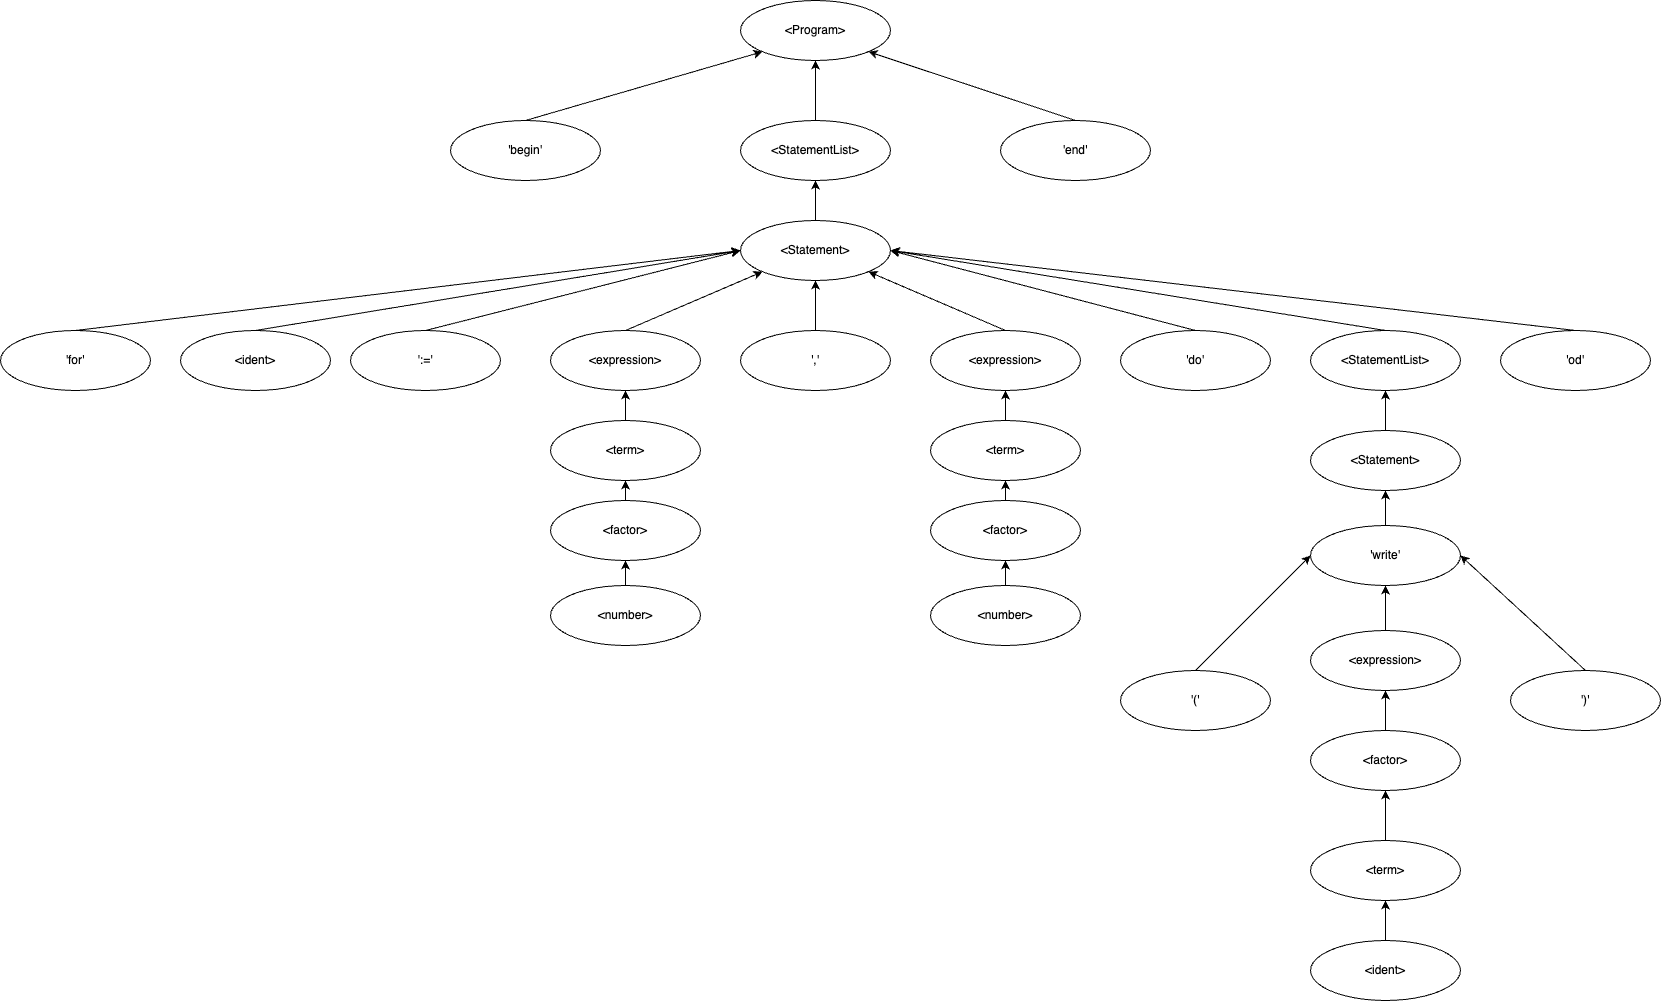
\includegraphics[width=0.9\textwidth]{tree.png}
    \caption{Дерево разбора}
\end{figure}

\newpage
\section{Трансляционные правила}

Обозначим:  
$addr(X)$ — адрес переменной цикла,  
$\ell$ — временная ячейка для предела,  
$\sigma$ — ячейка шага,  
$gen(\cdot)$ — операция «сгенерировать команду VM».

\subsection{Шаблон генерации p-кода для цикла}

\[
\begin{array}{@{}l@{\quad}l@{}}
\textbf{Инициализация:} &
  \mathrm{gen}(E_0),\;
  \mathrm{gen}(\mathrm{STORE},addr(X)), \\[2pt]
& \mathrm{gen}(E_f),\;
  \mathrm{gen}(\mathrm{STORE},\ell), \\[2pt]
& \mathrm{gen}\bigl(E_s\ \text{или}\ \mathrm{PUSH}\,1\bigr),\;
  \mathrm{gen}(\mathrm{STORE},\sigma) \\[6pt]

\textbf{Условие:} &
  cond \gets \text{addr текущей команды}, \\ 
& \mathrm{gen}(\mathrm{LOAD},addr(X)),\;
  \mathrm{gen}(\mathrm{LOAD},\ell),\;
  \mathrm{gen}(\mathrm{COMPARE},\le), \\ 
& j \gets \mathrm{gen}\!\bigl(\text{\texttt{JUMP\_NO}},\mathit{Exit}\bigr) \\[6pt]

\textbf{Тело цикла:} &
  \ldots\ \mathrm{gen}(p\text{-код списка }S)\ \ldots \\[6pt]

\textbf{Инкремент:} &
  \mathrm{gen}(\mathrm{LOAD},addr(X)),\;
  \mathrm{gen}(\mathrm{LOAD},\sigma),\;
  \mathrm{gen}(\mathrm{ADD}), \\ 
& \mathrm{gen}(\mathrm{STORE},addr(X)),\;
  \mathrm{gen}(\mathrm{JUMP},cond), \\ 
& \mathrm{gen}_{\text{at}}\bigl(j,\text{\texttt{JUMP\_NO}},\mathit{Exit}\bigr)
\end{array}
\]
  
\subsection{FIRST/FOLLOW}

Для доказательства единственности выбора продукции
рассчитаем множества $\mathrm{FIRST}$ и $\mathrm{FOLLOW}$
нетерминала \verb|<statement>|.

\paragraph{Множество FIRST}

\[
\begin{aligned}
\mathrm{FIRST}(\langle statement\rangle)=
\{&\textit{id},\
  \texttt{if},\
  \texttt{while},\
  \texttt{for},\
  \texttt{write} \}
\end{aligned}
\]

Каждый элемент отвечает уникальной продукции,  
поэтому $\mathrm{FIRST}$-множество альтернатив поп pairwise disjoint.

\paragraph{Множество FOLLOW}

\[
\mathrm{FOLLOW}(\langle statement\rangle)=
\{\texttt{;},\ \texttt{else},\ \texttt{fi},\ \texttt{od},\ \texttt{end}\}
\]

Получено стандартным алгоритмом, учитывая,
что \verb|<statementList>|~$\Rightarrow^*$~\verb|<statement>|.

\paragraph{Условие LL(1)}

Для двух альтернатив $A\to\alpha\mid\beta$ необходимо  
$\mathrm{FIRST}(\alpha)\cap\mathrm{FIRST}(\beta)=\varnothing$;  
эти множества приведены выше и не пересекаются.
Комплекты
$\mathrm{FIRST}(\alpha)\cap\mathrm{FOLLOW}(A)$
также пусты, так как $\varepsilon$-продукции отсутствуют.
Следовательно, конфликтов в парсинговой таблице нет,
и грамматика остаётся LL(1).

\begin{table}[H]
\centering\small
\caption{Фрагмент таблицы после расширения}
\begin{tabular}{|c|c|c|c|c|c|}
\hline
             & \textit{id} & \texttt{if} & \texttt{while} & \texttt{for} & \texttt{write} \\
\hline
\verb|<statement>| &
$\;X:=E\;$ &
\texttt{if}… &
\texttt{while}… &
\texttt{for}… &
\texttt{write}(E) \\
\hline
\end{tabular}
\end{table}

% -----------------------------------------------------------------
\newpage
\section{Новые токены}
Для расширения грамматики и поддержки цикла \texttt{for} были добавлены новые токены в лексический анализатор и грамматику языка Милан:

\begin{itemize}
    \item \textbf{T\_FOR}~--- ключевое слово \texttt{for}. Используется для распознавания начала конструкции цикла for. В грамматике инициирует разбор соответствующей продукции:
    \begin{verbatim}
    <statement> ::= ... | 'for' <ident> ':=' <expression> ',' <expression> [',' 
    
    <expression>] 'do' <statementList> 'od' | ...
    \end{verbatim}

    \item \textbf{T\_COMMA}~--- символ запятой (\texttt{,}). Используется для разделения начального значения, конечного значения и (опционально) шага в заголовке цикла for.

    \item \textbf{T\_DO}, \textbf{T\_OD}~--- ключевые слова \texttt{do} и \texttt{od}. Обозначают начало и конец тела цикла (и других управляющих конструкций).

    \item \textbf{T\_ASSIGN}~--- символ присваивания (\texttt{:=}). Используется для задания значения переменной цикла.

    \item \textbf{T\_IDENTIFIER}~--- идентификатор переменной (имя переменной цикла).

    \item \textbf{T\_NUMBER}~--- числовая константа (используется в выражениях).

    \item \textbf{T\_WRITE}, \textbf{T\_READ}~--- ключевые слова для ввода/вывода.

    \item \textbf{T\_BEGIN}, \textbf{T\_END}~--- ключевые слова для начала и конца программы.

    \item \textbf{T\_IF}, \textbf{T\_THEN}, \textbf{T\_ELSE}, \textbf{T\_FI}~--- ключевые слова для условных операторов.

    \item \textbf{T\_WHILE}~--- ключевое слово для цикла while.

    \item \textbf{T\_SEMICOLON}, \textbf{T\_LPAREN}, \textbf{T\_RPAREN}~--- служебные символы (точка с запятой, скобки).
\end{itemize}

\textbf{Пример использования новых токенов в грамматике:}

\begin{verbatim}
begin
    for i := 1, 10, 2 do
        write(i)
    od
end
\end{verbatim}

Здесь лексер выделяет следующие токены:
\begin{verbatim}
T_FOR T_IDENTIFIER T_ASSIGN T_NUMBER T_COMMA T_NUMBER T_COMMA T_NUMBER T_DO

T_WRITE T_LPAREN T_IDENTIFIER T_RPAREN T_OD
\end{verbatim}

Каждый из этих токенов участвует в разборе соответствующих продукций грамматики, обеспечивая корректную работу синтаксического анализатора и генерацию p-кода для новых конструкций языка.
    
\newpage
\section{Генерируемый p-код}
    
    Для программы
    \begin{lstlisting}[basicstyle=\small\ttfamily]
    begin
        for i := 1, 5 do
            write(i)
        od
    end
    \end{lstlisting}
    компилятор выдаёт:
    
    \begin{verbatim}
    0:  PUSH    1
    1:  STORE   0         ; i := 1
    2:  PUSH    5
    3:  STORE   1         ; limit
    4:  PUSH    1
    5:  STORE   2         ; step
    6:  LOAD    0
    7:  LOAD    1
    8:  COMPARE 4         ; <=
    9:  JUMP_NO 19
    10: LOAD    0
    11: PRINT
    12: LOAD    0
    13: LOAD    2
    14: ADD
    15: STORE   0
    16: JUMP    6
    19: STOP
    \end{verbatim}
    \newpage
    \section{Тестовые примеры}
    
    \begin{enumerate}
      \item \textbf{demo2.mil}
    \begin{lstlisting}
    begin
        for k := 5, 5 do
            write(k)
        od
    end
    \end{lstlisting}
      Вывод: \texttt{5}
    
      \item \textbf{demo3.mil}
    \begin{lstlisting}
    begin
        for x := 2, 8, 3 do
            write(x)
        od
    end
    \end{lstlisting}
      Вывод: \texttt{2 5 8}

      \item \textbf{demo4.mil} (Вложенный цикл)
      \begin{lstlisting}
      begin
          for i := 1, 3 do
              for j := 1, 2 do
                  write(i)
                  write(j)
              od
          od
      end
      \end{lstlisting}
      Вывод: \texttt{1 1 1 2 2 1 2 2 2}

      \item \textbf{demo5.mil} (Отрицательная итерация)
      \begin{lstlisting}
      begin
          for k := 5, 1, -2 do
              write(k)
          od
      end
      \end{lstlisting}
      Вывод: \texttt{5 3 1}
    \end{enumerate}
    \newpage
    \section{Инструкция по запуску}
    
    \begin{enumerate}
      \item \textbf{Сборка компилятора}\\
            \lstinline|cd cmilan/src && make|
      \item \textbf{Компиляция исходников}\\
            \lstinline|./cmilan ../test/demo2.mil > ../../demo2.asm|
      \item \textbf{Сборка виртуальной машины}\\
            \lstinline|cd ../../vm/vm && make|
      \item \textbf{Запуск программы}\\
            \lstinline|./mvm ../../demo2.asm|
    \end{enumerate}
    \newpage
    \section*{Заключение}
    \addcontentsline{toc}{section}{Заключение}
    
    В ходе работы грамматика языка Милан была расширена,
    а компилятор \textbf{CMilan} модифицирован для поддержки счётного
    цикла~\texttt{for}.  
    Добавлены два токена (\texttt{T\_FOR}, \texttt{T\_COMMA}) и
    одна продукция грамматики; изменены файлы
    \lstinline{scanner.h/.cpp} и \lstinline{parser.cpp}.
    FIRST/FOLLOW-анализ подтвердил, что грамматика осталась LL(1),
    а семантические схемы гарантируют корректную генерацию~p-кода.
    Тестовые программы успешно выполняются на виртуальной машине,
    что демонстрирует отсутствие регрессий в существующем функционале.
    Реализованы вложенные циклы. 
    
    \subsection*{Плюсы}
    \begin{itemize}
      \item \textbf{Минимальные правки.}  Лексер и парсер дополнены точечно;
            остальной код и интерфейсы остались неизменными.
      \item \textbf{Поддержка отрицательных итераций.} Так же реализованы циклы с обратным шагом.
    \end{itemize}
    
    \subsection*{Минусы}
    \begin{itemize}
      \item \emph{Нет проверки знака шага.}  Если итерация указан нулём,
            цикл становится бесконечным ― на уровне компиляции это
            не диагностируется.
      \item \emph{Только линейный счётчик.}  Условие окончания жёстко
            «$\le$» или «$\ge$» в зависимости от знака шага; более
            сложные предикаты (например, \texttt{while i*i<n}) требуют
            обычного~\texttt{while}.
      \item \emph{Отсутствие поддержки \texttt{break}/\texttt{continue}.}
            Досрочный выход из цикла не предусмотрен.
    \end{itemize}
    
    \subsection*{Дополнение}
    \begin{itemize}
      \item Добавить статическую проверку <<итерация $\neq 0$>> и предупреждение
            о неверном направлении счётчика.
      \item Реализовать ключевые слова \texttt{break} и \texttt{continue}
            с генерацией соответствующих \texttt{JUMP}-инструкций.
      \item Поддержать диапазонный синтаксис\,:  
            \verb|for i in 1..10 [step 2] do ... od|.
      \item Расширить виртуальную машину новым сравнением
            «$>$= / $<$= с шагом $\pm1$» для компактного p-кода.
    \end{itemize}
    
\newpage
\section*{Список литературы}
\addcontentsline{toc}{section}{Список литературы}
\begin{enumerate}
    \item Ю.Г. Карпов, Теория и технология программирования. Основы построения
    трансляторов. СПб.: БХВ-Петербург, 2005.
    \item А. Ахо, М. Лам, Р. Сети, Дж. Ульман, Компиляторы: принципы, технологии и
    инструментарий, 2-е изд. М.: Вильямс, 2011.
\end{enumerate}
\end{document}